This project is a swedish question answering system developed in the course EDAN70 at LTH.
The goal is to create a system that is able to answer questions with one word long answers.
To do this, the swedish wikipedia was used as data source, and the annotated questions from the swedish 
board game Kvitt eller dubbelt was used as training questions and categories.

A fundamental system overview is shown in figure \ref{fig:overview}. 

\begin{figure*}
\centering
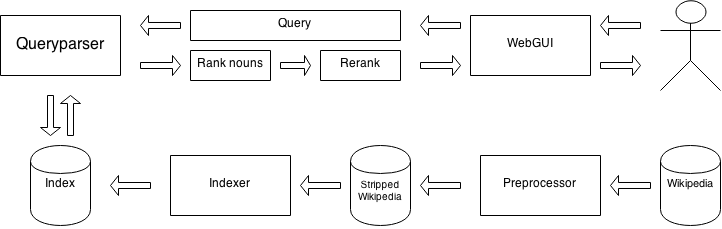
\includegraphics[width=1\textwidth]{figures/Question-answering-system.png}
\caption{Overview}
\label{fig:overview}
\end{figure*}
